\documentclass[12pt]{article}
\usepackage{graphicx}
\usepackage{amsmath}
\usepackage{amssymb}
\usepackage{float}
\usepackage{commath}
\usepackage{siunitx}
\sisetup{detect-all}
\usepackage[a4paper,width=160mm,top=20mm,bottom=20mm]{geometry}
\numberwithin{equation}{section}
\setlength{\parskip}{\baselineskip}%
\setlength{\parindent}{0pt}%
\begin{document}
\title{\textbf{UCL Mechanical Engineering 2020/2021}\\MECH0010 Coursework 1}
\date{Starting on: 31/10/2020\\Deadline: 13/11/2020}
\author{Anonymous submission}
\maketitle
\tableofcontents
\newpage
\part{Control}
\section{Question A}
\subsection*{Block diagram (open loop)}
\begin{figure}[H]
  \centering
  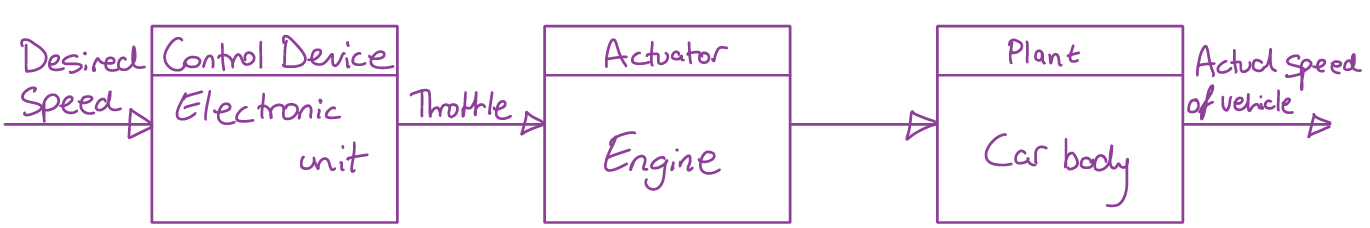
\includegraphics[width=\textwidth]{./img/1-1blockdiagram.png}
\end{figure}
\subsection*{Block diagram (closed loop)}
\begin{figure}[H]
  \centering
  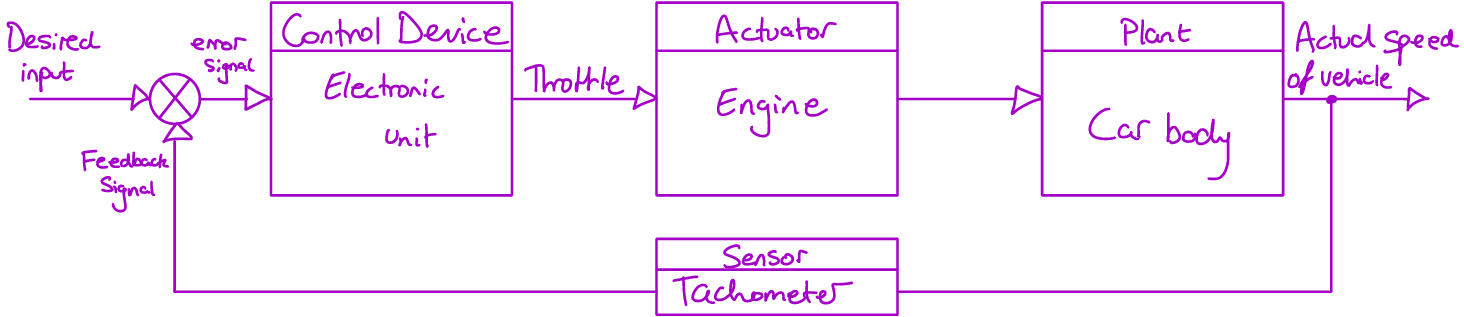
\includegraphics[width=\textwidth]{./img/1-2blockdiagram.png}
\end{figure}
With closed loop control, we can better control the actual speed of the vehicle. For example, when in abnormal conditions, (bad weather, incline, decline) there will be a different resistive force acting against the motion of the vehicle. In the cases where the resistance force is changed, the speed of the vehicle will change, if power output is constant (assuming throttle position is proportional to engine power output). 

For example, on an incline not only does the engine force have to match the resistive forces but also the sine component of the weight of the vehicle ($\sum{\textrm{opposing forces}} = F_R + mg\sin{\theta}$, where $\theta$ is the incline angle.) The derivation for the equation linking power output, force and velocity is below.
\begin{align}
  W &= \int_{x_0}^{x} F \cdot \textrm{d}x\\
  v &= \frac{\dif x}{\dif t}\\
  v\dif t &= \dif x\\
  W &= \int_{t_0}^{t} Fv\cdot \textrm{d} t\\
  P &= \frac{\dif W}{\dif t}\\
  P &= \frac{\dif}{\dif t}\left(\int_{t_0}^{t} Fv\cdot \textrm{d} t\right)\\
  P &= Fv
\end{align}
If $P$ is constant and $F$ is increased/decreased, $v$ must decrease/increase.
\subsection*{Proximity sensors}
We can utilise a proximity sensor to measure the distance to the vehicle ahead. This can be used to 'track' the vehicle ahead. A simple cruise control system is unable to make changes to the throttle in response to changing road conditions. With a proximity sensor, we can observe whether the vehicle ahead is getting closer (vehicle ahead is braking) or moving further away (vehicle ahead is accelerating away). By setting a fixed 'following distance' (how far away the vehicle ahead should be kept), the driver can set a maximum speed for the vehicle to travel at and the vehicle will automatically slow down and speed up to the limits set in response to changing road conditions. 

For example, in traffic vehicles are constantly slowing down and accelerating. With our previous system, we would have to disable the cruise control (by braking) and set it again once vehicles speed up again. Our new system will allow a user to simply set the cruise control once and no longer worry about colliding into the car in front, as the car will keep a safe distance from the vehicle.
\section{Question B}
\begin{itemize}
  \item Sensor - circuit to measure resistance of heating coil.
  \item Actuator - heating element
  \item Input signal(s)
    \begin{itemize}
      \item Relay switch (heating element on and off, convection fan on and off)
      \item Rotary switch (temperature control)
    \end{itemize}
  \item Output signal(s) - temperature
  \item Control signal(s) - 
\end{itemize}
\begin{figure}[H]
  \centering
  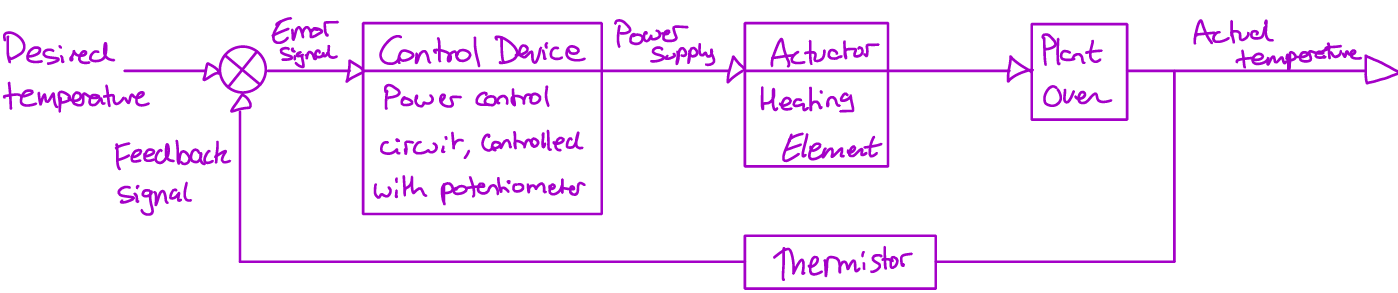
\includegraphics[width=\textwidth]{./img/2-1blockdiagram.png}
\end{figure}
My first solution is to have an open-loop control system. Our input is simply the temperature desired. I have left the timing to an external device such as an oven timer, however this could be easily implemented with a simple timing circuit and relay. This system utilises a potentiometer as an analogue input. Each resistance setting corresponds to a certain desired temperature. Our heating element operates on the basis of Joule heating, whereby passing a current through a conductor produces a heating effect. Assuming that the heating element is a perfect resistor, we know that:
\begin{align}
  P &= IV\\
  V &= IR\\
  I &= \frac{V}{R}\\
  P &= I^2 \cdot R
\end{align}
Whether we use a DC supply or an AC supply has a negligible effect on our system, as we can simply look at the RMS values for AC. 

Our heating element will continue to heat up until it reaches a certain equilibrium (where the power in to the heating element matches the heat dissipation), however this equilibrium temperature will most likely not be the desired temperature. We have two options here: modulate our power supply to change the equilibrium temperature of the heating element or switch the power supply off and on at threshold values. Some of the advantages of power modulation include a stable temperature, but this may come at the cost of additional electronic complexity and cost. 

On the other hand, on-off control is relatively simple. We can set our threshold values to be $\pm 5\si{\celsius}$ of the desired temperature. I have arbitrarily chosen this value, as the the effects of a temperature oscillation of 10\si{\celsius} will have negligible effects on the food being cooked. The thermal inertia of the heating coil is also relatively high, thus switching will occur with low frequency and can be managed with a simple relay.
\begin{figure}[H]
  \centering
  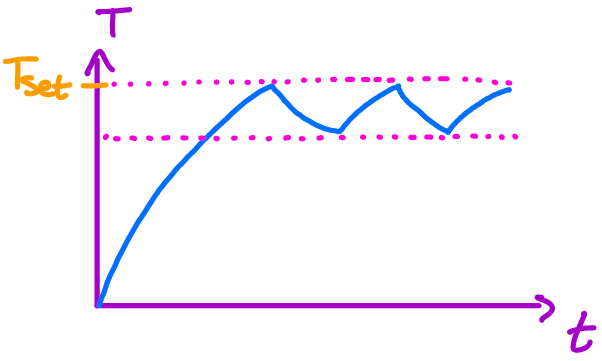
\includegraphics[width=0.6\textwidth]{./img/2-2graph.png}
  \caption{Temperature - time graph for an on-off control system. We can see the desired temperature as $T_{set}$ and our threshold temperatures as the pink dotted lines. As the circuit is switched on and off, the temperature of the oven is controlled.}
\end{figure}
\begin{figure}[H]
  \centering
  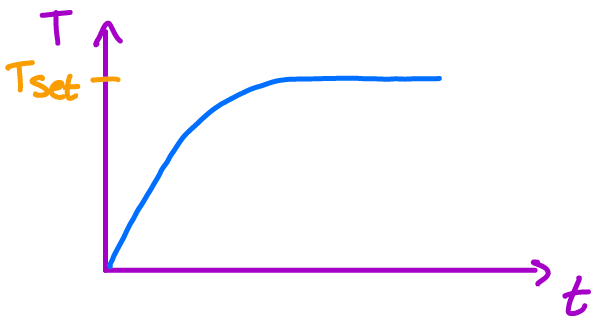
\includegraphics[width=0.6\textwidth]{./img/2-3graph.png}
  \caption{Temperature - time graph for a modulated power supply. Here we can see that the equilibrium temperature is our $T_{set}$ value - the temperature at which power in = power dissipated.}
\end{figure}
\section{Question C}
\subsection*{Transfer function}
\begin{figure}[H]
  \centering
  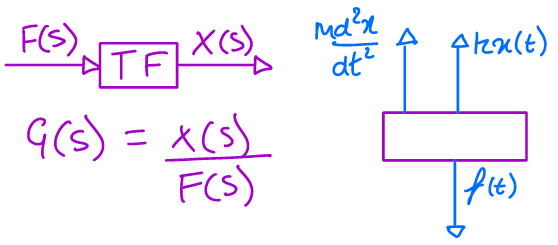
\includegraphics[width=0.6\textwidth]{./img/2-4blockdiagram.png}
\end{figure}
\begin{align}
  G(s) &= \frac{X(s)}{F(s)}\\
  f(t) &= kx(t) + m \frac{\dif ^2 x}{\dif t^2}\\
  F(s) &= kX(s) + ms^2 X(s)\\
  F(s) &= X(s) (k + ms^2)\\
  \frac{X(s)}{F(s)} &= \frac{1}{k + ms^2}\\
  \frac{X(s)}{F(s)} &= \frac{\frac{1}{m}}{s^2 + \frac{k}{m}}
\end{align}
\subsection*{Time domain response}

\begin{align}
  \frac{X(s)}{F(s)} &= \frac{\frac{1}{m}}{s^2 + \frac{k}{m}}\\
  \frac{X(s)}{F(s)} &= \frac{\sqrt{\frac{k}{m}}}{s^2 + \frac{k}{m}} \times \frac{1}{\sqrt{mk}}
\end{align}
Where $\omega = \sqrt{\frac{k}{m}}$
\begin{align}
  x(t) = L^{-1} \left[ \frac{\sqrt{\frac{k}{m}}}{s^2 + \frac{k}{m}} \cdot \frac{1}{\sqrt{mk}} \right]\\
  x(t) = \frac{1}{\sqrt{mk}} \cdot L^{-1} \left[ \frac{\sqrt{\frac{k}{m}}}{s^2 + \frac{k}{m}} \right]\\
  x(t) = \frac{1}{\sqrt{mk}} \cdot \sin{\left(\sqrt{\frac{k}{m}}\cdot t\right)}
\end{align}
\begin{figure}[H]
  \centering
  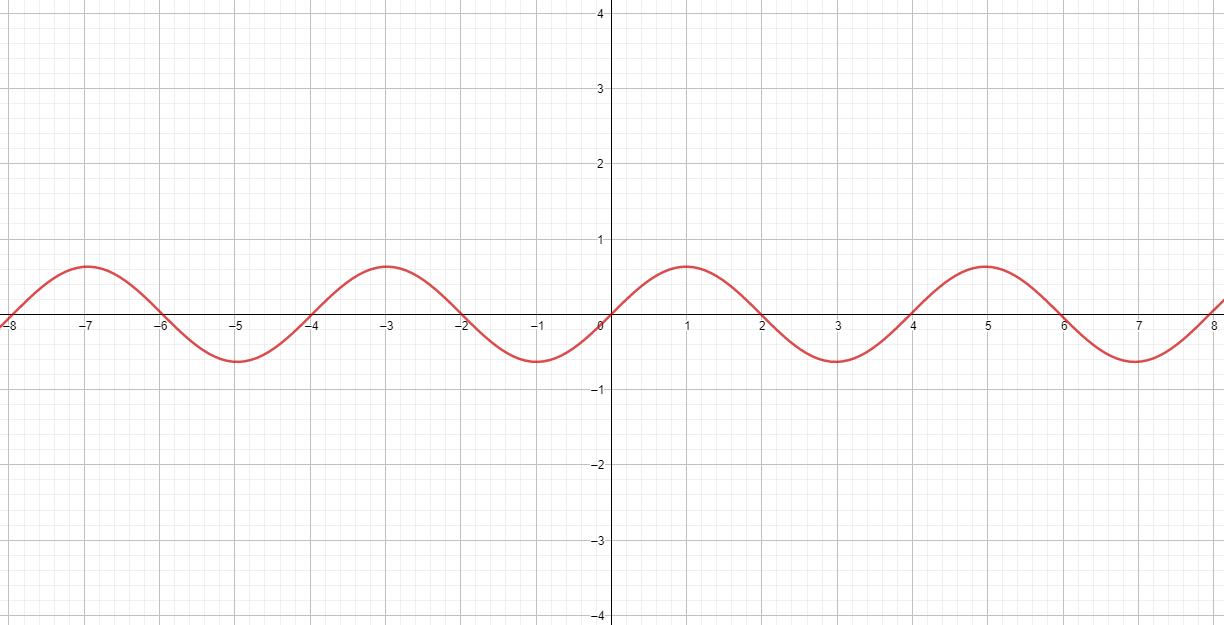
\includegraphics[width=\textwidth]{./img/3-1timeresponse.png}
  \caption{Graph to show plot of $x(t) = \frac{1}{\sqrt{mk}} \cdot \sin{\left(\sqrt{\frac{k}{m}}\cdot t\right)}$. $m$ and $k$ were arbitrarily selected as 1 and 2.5 respectively. When $m$ is increased/decreased, we see the frequency and gain increase/decrease. When $k$ is increased/decreased, we see the frequency }
\end{figure}
\part{Instrumentation}
\section{Question 1}
\subsection*{Wheatstone bridge}
\begin{figure}[H]
  \centering
  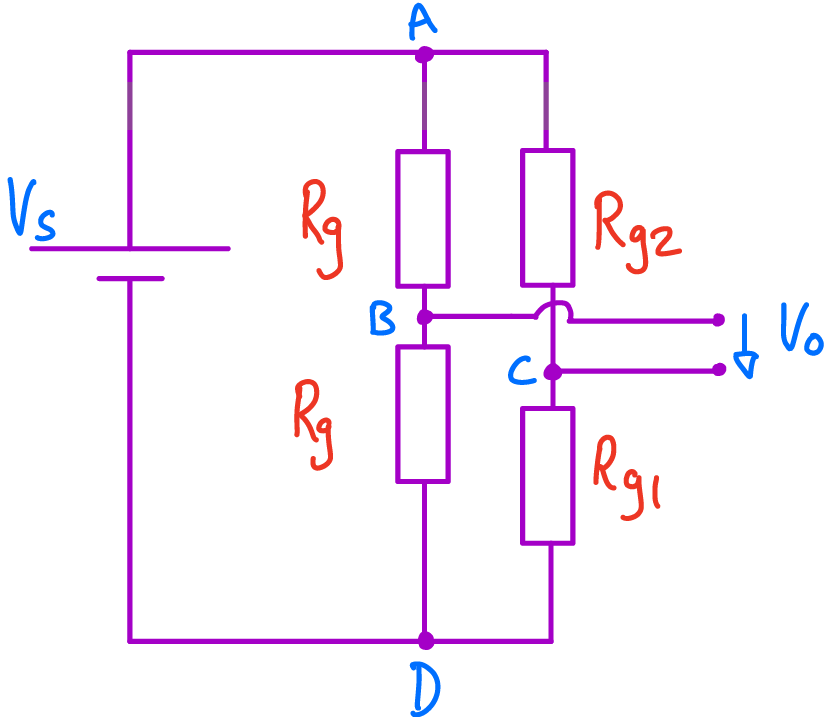
\includegraphics[width=0.4\textwidth]{./img/4-1circuit.png}
  \caption{Circuit diagram to show a Wheatstone bridge}
\end{figure}
We know that:
\begin{align}
  V_0 &= V_S \left( \frac{R_{g1}}{R_{g1} + R_{g2}} - \frac{1}{2} \right)\\
  V_0 &= V_S \frac{R(1+x)}{R(1+x) + R(1-x)} - \frac{V_S}{2}\\
  V_0 &= \frac{1}{2} V_S \cdot x
\end{align}
We know that $x = eG$, hence:
\begin{equation}
  \frac{V_0}{e} = \frac{1}{2}V_S \cdot G
\end{equation}
\subsection*{Identify specification}
\begin{itemize}
  \item $G = 2.1$
  \item $R_g = 120\si{\ohm}$
  \item $\frac{V_0}{e} = 5\si{\volt}$
\end{itemize}
\begin{align}
  5 &= \frac{1}{2} V_S \times 2.1\\
  V_S &= 4.8 \si{\volt} \textrm{ (2sf)}\\
  R = R_g &= 120\si{\ohm}
\end{align}
\subsection*{Longitudinal stretch}
Since the strain gauges are being stretched on a perpendicular axis, the strain in the wires will become a negligible quantity. This will lead to an approximately 0 $V_S$. 
\begin{align}
  V_0 &= V_S \left( \frac{R_{g1}}{R_{g1} + R_{g2}} - \frac{1}{2} \right)\\
  R_{g1} &= R_{g2} = R(1+x)\\
  V_0 &= V_S\frac{R(1+x)}{2R(1+x)} - \frac{V_S}{2}\\
  V_0 &= 0 
\end{align}
\subsection*{Method to increasing sensitivity}
\begin{figure}[H]
  \centering
  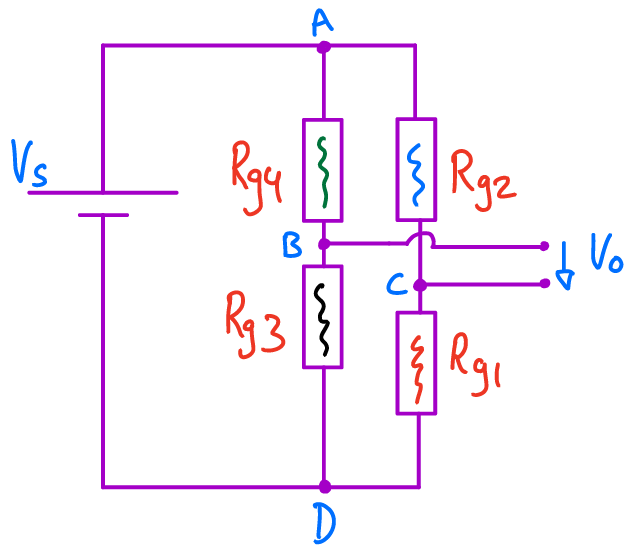
\includegraphics[width=0.4\textwidth]{./img/4-4circuit.png}
  \caption{Circuit diagram to show a Wheatstone bridge with increased sensitivity.}
\end{figure}
\begin{figure}[H]
  \centering
  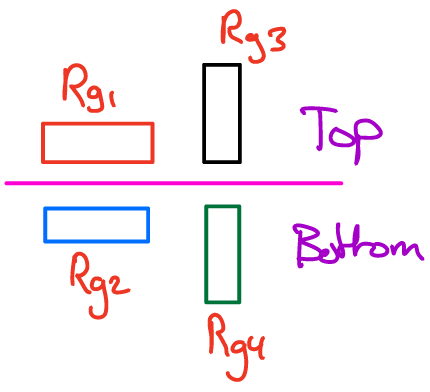
\includegraphics[width=0.4\textwidth]{./img/4-4arrangement.png}
  \caption{Diagram to show arrangement of strain gauges for increased sensitivity.}
\end{figure}
\begin{align}
  V_0 &= V_S \left(\frac{R_{g1}}{R_{g1} + R_{g2}} - \frac{R_{g3}}{R_{g3} + R_{g4}}\right)\\
  V_0 &= V_S \left(\frac{R(1+x)}{R(1+x) + R(1+\nu x)} - \frac{R(1-\nu x)}{R(1-\nu x) + R(1+\nu x)}\right)\\
  V_0 &= V_S \left(\frac{1}{2}(1+x) - \frac{1}{2}(1-\nu x)\right)\\
  V_0 &= \frac{V_S \cdot x}{2} \left(1 + \nu \right)\\
  \frac{V_0}{e} &= \frac{4.8}{2} \times 2.1\times  (1 + 0.3)\\
  \frac{V_0}{e} &= 6.6 \si{\volt}
\end{align}
$6.6 > 5$, hence we can see that this arrangement has increased sensitivity.
\section{Question 2}
\section{Question 3}
\end{document}